\documentclass[11pt]{article}
\usepackage[margin=1in]{geometry}
\usepackage{clrscode3e}
\usepackage{amsmath,amsthm,amssymb}
\usepackage{mathtools}
\usepackage{tikz}
\usepackage{float}
\usetikzlibrary{positioning,arrows}
\usepackage{setspace}
\usepackage{mathpazo}
\doublespacing
%\usepackage{tikz-berge}
%\usepackage{algorithm}
%\usepackage[noend]{algpseudocode}

 
\newcommand{\N}{\mathbb{N}}
\newcommand{\Z}{\mathbb{Z}}
\newcommand{\R}{\mathbb{R}}
\renewcommand{\'}{^{'}}
\renewcommand{\gets}{:=}
 
\newenvironment{theorem}[2][Theorem]{\begin{trivlist}
\item[\hskip \labelsep {\bfseries #1}\hskip \labelsep {\bfseries #2.}]}{\end{trivlist}}
\newenvironment{lemma}[2][Lemma]{\begin{trivlist}
\item[\hskip \labelsep {\bfseries #1}\hskip \labelsep {\bfseries #2.}]}{\end{trivlist}}
\newenvironment{definition}[2][Definition]{\begin{trivlist}
\item[\hskip \labelsep {\bfseries #1}\hskip \labelsep {\bfseries #2.}]}{\end{trivlist}}
\newenvironment{problem}[2][Problem]{\begin{trivlist}
\item[\hskip \labelsep {\bfseries #1}\hskip \labelsep {\bfseries #2.}]}{\end{trivlist}}
\newenvironment{question}[2][Question]{\begin{trivlist}
\item[\hskip \labelsep {\bfseries #1}\hskip \labelsep {\bfseries #2.}]}{\end{trivlist}}

\begin{document}
\title{Chapter 1}
\author{Zachary Campbell}

\maketitle

\begin{section}{Introduction}
	This thesis is aimed at those who have taken a course in algorithms, especially one in which 
	network flows, and the max-flow/min-cut theorem were discussed. In this introductory chapter 
	I will review these topics more briefly, and discuss their relevance to this thesis. 
	We are not discussing flows or cuts in this thesis (although much of the work done in this 
	thesis has a shifted frame of reference via flows), but their relevance will be made clear. 
	The most important thing for the reader to have is a curiosity about the max-flow/min-cut 
	theorem; there is a lot of cool math behind it, and we demonstrate that math in other settings. 
	Specifically, we look at this relationship in weighted bipartite matchings.
\end{section}

\begin{section}{Bipartite graphs and matchings}

	Throughout this thesis we will be interested in a specific subclass of graphs known as 
	bipartite graphs. Unless otherwise noted, our algorithms will assume a bipartite structure.

	\begin{definition}{(Bipartite graph)}
		A \emph{bipartite graph} is a graph whose vertices can be partitioned into two 
		sets $U$ and $V$ such that all edges connect a vertex $u\in U$ to a vertex $v\in V$.
		We will denote this graph $G = (U,V,E)$, where $E$ is the edge set $(U\times V)$.
	\end{definition}
	
	\begin{figure}[h]
		\centering
	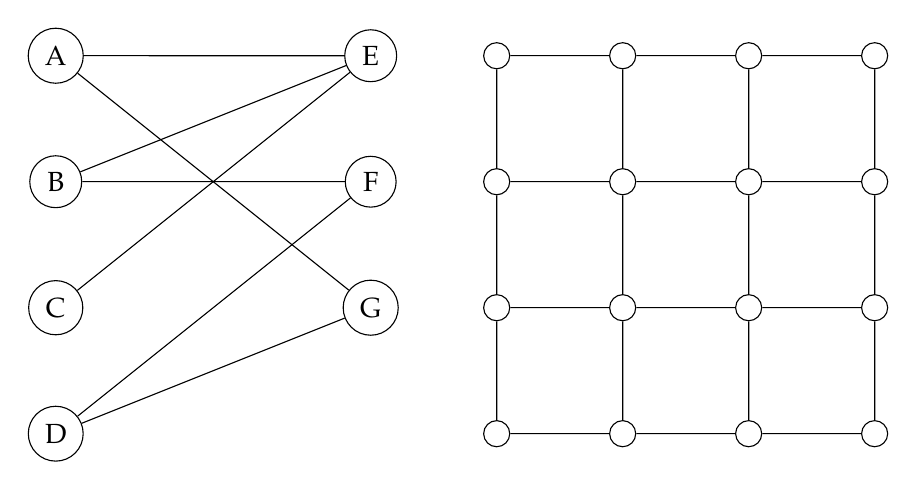
\begin{tikzpicture}[scale=.8,auto=left,every node/.style={circle,draw=black}]
		%left nodes
		\node (n1) at (1,10) {A};
		\node (n2) at (1,8) {B};
		\node (n3) at (1,6) {C};
		\node (n4) at (1,4) {D};

		%right nodes
		\node (n5) at (6,10) {E};
		\node (n6) at (6, 8) {F};
		\node (n7) at (6, 6) {G};
		
		%edges
		\draw (n1) -- (n5);
		\draw (n1) -- (n7);
		\draw (n2) -- (n5);
		\draw (n2) -- (n6);
		\draw (n3) -- (n5);
		\draw (n4) -- (n6);
		\draw (n4) -- (n7);

		%left nodes
		\node (n1) at (8,10) {};
		\node (n2) at (8,8) {};
		\node (n3) at (8,6) {};
		\node (n4) at (8,4) {};

		%center left nodes
		\node (n5) at (10,10) {};
		\node (n6) at (10,8) {};
		\node (n7) at (10,6) {};
		\node (n8) at (10,4) {};

		%center right nodes
		\node (n9) at (12,10) {};
		\node (n10) at (12,8) {};
		\node (n11) at (12,6) {};
		\node (n12) at (12,4) {};

		%right nodes
		\node (n13) at (14,10) {};
		\node (n14) at (14,8) {};
		\node (n15) at (14,6) {};
		\node (n16) at (14,4) {};

		%edges
		\draw (n1) -- (n2);
		\draw (n1) -- (n5);
		\draw (n2) -- (n3);
		\draw (n2) -- (n6);
		\draw (n3) -- (n4);
		\draw (n3) -- (n7);
		\draw (n4) -- (n8);
		\draw (n5) -- (n6);
		\draw (n5) -- (n9);
		\draw (n6) -- (n7);
		\draw (n6) -- (n10);
		\draw (n7) -- (n8);
		\draw (n7) -- (n11);
		\draw (n8) -- (n12);
		\draw (n9) -- (n10);
		\draw (n9) -- (n13);
		\draw (n10) -- (n11);
		\draw (n10) -- (n14);
		\draw (n11) -- (n12);
		\draw (n11) -- (n15);
		\draw (n12) -- (n16);
		\draw (n13) -- (n14);
		\draw (n14) -- (n15);
		\draw (n15) -- (n16);
	\end{tikzpicture}
	\caption{Examples of bipartite graphs}
	\end{figure}

	In Figure 1 we have a bipartite graph with vertex partition given by $U = \{A,B,C,D\}$ and 
	$V = \{E,F,G\}$. All edges in this graph are between a node $u\in U$ and a node $v\in V$. The 
	graph on the right is also bipartite. It may take a little more time to convince yourself that 
	you can partition the vertices into disjoint $U$ and $V$ in a way that maintains the 
	bipartite property. Try it!
	Now that we know what we are working with, let's introduce a problem that 
	we'd like to solve on these graphs.  
	\begin{definition}{(Matching)}
		Let $G = (U,V,E)$ be a bipartite graph. A subset $M\subset E$ is a \emph{matching} if 
		no two edges in $M$ are incident to the same vertex. We call a matching 
		\emph{perfect} if all vertices are an endpoint of an edge in $M$.
	\end{definition}
	We say that a vertex $w\in U\cup V$ is \emph{matched} with respect to $M$ if it is an endpoint 
	of some edge in $M$. The following figure shows some examples of different matchings on one 
	of the graphs from Figure 1.

	\begin{figure}[h]
		\centering
		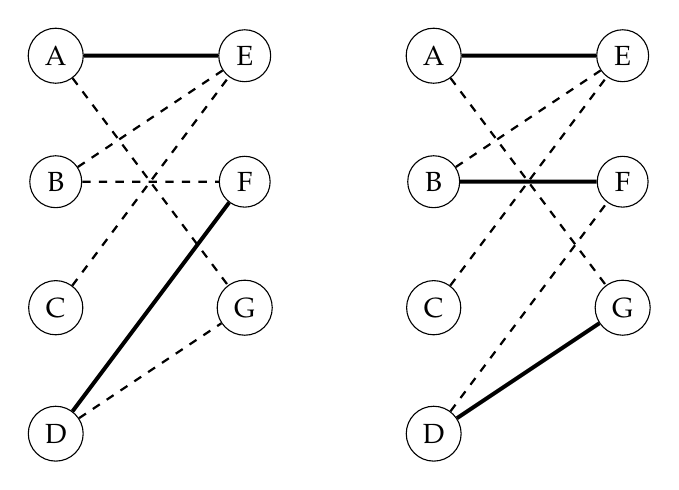
\begin{tikzpicture}[scale=.8,auto=left,every node/.style={circle,draw=black}]
		
		%left nodes
		\node (n1) at (1,10) {A};
		\node (n2) at (1,8) {B};
		\node (n3) at (1,6) {C};
		\node (n4) at (1,4) {D};

		%right nodes
		\node (n5) at (4,10) {E};
		\node (n6) at (4, 8) {F};
		\node (n7) at (4, 6) {G};
		
		%edges
		\draw[line width=0.5mm] (n1) -- (n5);
		\draw[thick,dashed] (n1) -- (n7);
		\draw[thick,dashed] (n2) -- (n5);
		\draw[thick,dashed] (n2) -- (n6);
		\draw[thick,dashed] (n3) -- (n5);
		\draw[line width=0.5mm] (n4) -- (n6);
		\draw[thick,dashed] (n4) -- (n7);

		%left nodes
		\node (m1) at (7,10) {A};
		\node (m2) at (7,8) {B};
		\node (m3) at (7,6) {C};
		\node (m4) at (7,4) {D};

		%right nodes
		\node (m5) at (10,10) {E};
		\node (m6) at (10, 8) {F};
		\node (m7) at (10, 6) {G};
		
		%edges
		\draw[line width=0.5mm] (m1) -- (m5);
		\draw[thick,dashed] (m1) -- (m7);
		\draw[thick,dashed] (m2) -- (m5);
		\draw[line width=0.5mm] (m2) -- (m6);
		\draw[thick,dashed] (m3) -- (m5);
		\draw[thick,dashed] (m4) -- (m6);
		\draw[line width = 0.5mm] (m4) -- (m7);

		\end{tikzpicture}
		\caption{Examples of matchings on a bipartite graph}
	\end{figure}

	There many different valid matchings on the graph in Figure 2. Oftentimes, we want to find 
	the largest matching on a graph. This is classically motivated by economic examples, where we 
	have a set of bidders, and a set of goods, and the edges between them denote a bidder $i$'s 
	willingness to pay for good $j$. For a money-hungry auctioneer, the goal here would be to 
	find the ``largest'' matching on the graph, i.e. the one that maximizes profit of the auction. 
	We will discuss this interpretation in more depth later on in the thesis.
	This leads to the following definition.
	\begin{definition}{(Maximal matching)}
		A \emph{maximal matching} on $G$ is a matching $M$ such that if any other edge 
		not in $M$ is added to $M$, it is no longer a valid matching. Alternatively put, 
		$M$ is maximal if there is no matching $M\'$ such that $M\subset M\'$.
	\end{definition}
	Both matchings in Figure 2 are maximal matchings; in each case there are no edges that 
	we can add to $M$ and have that $M$ is still a matching. However, notice that the size of 
	the matchings is different, even though both are maximal on $G$. This leads to the following 
	definition.

	\begin{definition}{(Maximum matching)}
		A matching $M$ on a graph $G$ is said to be a \emph{maximum} matching if for all other 
		matchings $M\'$ on $G$, $|M\'| \leq |M|$.
	\end{definition}
	In our example, the matching on the right given by $M = \{(A,E), (B,F), (D,G)\}$ is a 
	maximum matching (convince yourself). In general there may be many unique maximum matchings 
	on a graph.\\
	In this section we are interested in general methods for finding maximum matchings on 
	bipartite graphs. One of the fundamental approaches is to look at certain subgraphs called 
	alternating paths. Before we define what these are, let's look at a motivating example.
	Suppose we have the matching on the left in Figure 2. So $M = \{(A,E),(D,F)\}$. Consider 
	the following sequence of vertices in the graph:

	\begin{figure}[h]
		\centering
		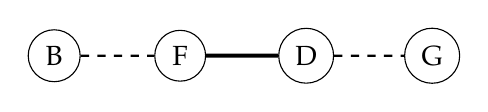
\begin{tikzpicture}[scale=.8,auto=left,every node/.style={circle,draw=black}]

			\node (n1) at (1,10) {B};
			\node (n2) at (3,10) {F};
			\node (n3) at (5,10) {D};
			\node (n4) at (7,10) {G};

			\draw[thick,dashed] (n1) -- (n2); 
			\draw[line width=0.5mm] (n2) -- (n3);
			\draw[thick,dashed] (n3) -- (n4);
		\end{tikzpicture}
	\end{figure}
	Call this sequence $p$. Let's perform an 
	operation that we will denote $M\oplus p$, which operates like XOR: add to $M$ each edge in 
	$p$ that isn't in $M$, and remove from $M$ each edge in $p$ that is in $M$. This gives us 
	the following segment, where $(B,F)$ and $(D,G)$ are now in $M$, but $(D,F)$ is not:

	\begin{figure}[h]
		\centering
		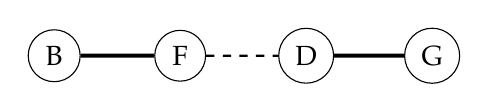
\begin{tikzpicture}[scale=.8,auto=left,every node/.style={circle,draw=black}]

			\node (n1) at (1,10) {B};
			\node (n2) at (3,10) {F};
			\node (n3) at (5,10) {D};
			\node (n4) at (7,10) {G};

			\draw[line width=0.5mm] (n1) -- (n2); 
			\draw[thick,dashed] (n2) -- (n3);
			\draw[line width=0.5mm] (n3) -- (n4);
		\end{tikzpicture}
	\end{figure}
	First, we must check that the new $M$ is still a valid matching; we do this by noticing that 
	$B$ and $G$ were originally unmatched, so it's okay for one of their incident edges to be 
	added. Also, notice that the size of our matching has grown by 1! In fact, this new matching 
	is exactly the matching given by the graph on the right in Figure 2. 
	This is a general technique in 
	finding maximum matchings. We want to look for these paths that start and end at unmatched 
	vertices, and whose edges are alternately matched and unmatched. If we can find one of these 
	paths, we will be able to increase the size of matching. We define this formally now.

	\begin{definition}{(Alternating path)}
		Let $G$ be a graph and $M$ some matching on $G$. An \emph{alternating path} is a 
		sequence of vertices and edges that begins with an unmatched vertex, and whose 
		edges alternate between being in $M$ and not in $M$.
	\end{definition}

	\begin{definition}{(Augmenting path)}
		An \emph{augmenting path} is an alternating path that starts and ends on unmatched 
		vertices. When we augment $M$ by an augmenting path $p$, we use the notation 
		$M\oplus p$.
	\end{definition}
	This motivates a general method for finding a maximum matching on a bipartite graph: 
	just keep looking for augmenting paths, and augment the current matching by that augmenting 
	path. Of course, we need to prove that this in fact gives us a maximum matching. The following 
	theorem says exactly that.

	\begin{theorem}{(Berge, 1957)}
		A matching $M$ on $G$ is a maximum matching if and only if $G$ contains no augmenting 
		paths with respect to $M$.
	\end{theorem}
	\singlespace
	This gives us the following framework for finding maximum matchings in bipartite graphs.
	\begin{codebox}
		\Procname{$\proc{Alg 1} (G) $}
		\li $M \gets \emptyset $
		\li $\While$ there exists an augmenting path $p$
			\Do
		\li		$M \gets M\oplus p$
			\End
		\li $\Return$ $M$
	\end{codebox}
	\doublespacing
	Note that we have yet to describe the details of this algorithm. Before we do so, we are going 
	to take a step back a bit and look at the maximum matching problem from a slightly different 
	perspective. In doing so, we will develop a language for talking about this problem that will 
	serve us throughout the rest of this thesis. At first, the approach will appear purely 
	pedagogic, but hopefully the reader will understand the significance of it by the end of the 
	thesis.

\end{section}

\begin{section}{Linear programming}
	The development of combinatorial optimization has been deeply intertwined with the discipline 
	of linear programming. In its most basic form, linear programs are given by some linear 
	objective function that you want to optimize, along with some linear constraint equations. 
	For a more detailed treatment on linear programming, we will refer you to (CITE LP SOURCES).
	For the purposes of this thesis, we will treat linear programming more casually, only requiring 
	a few key results. Moreover, we will not be discussing methods of actually solving linear 
	programs, for which there are at least a couple of well known but complicated algorithms. \\
	In the general linear-programming problem, our goal is to optimize some linear function that 
	is constrained by a set of linear inequalities. These problems are ubiquitous in applied math 
	and computer science, as they model a system in which something needs to be optimized according 
	to competing resources. We can express a general \emph{maximization} linear program as

	\begin{alignat}{3}
		& \text{maximize } & \sum_{j=1}^{n} c_{j} x_{j}& \\
		& \text{subject to } \quad & \sum_{j=1}^{n} a_{ij} x_{j} & \leq b_{j}, & i & = 1, \dots 
		, m \\
				&& x_{j} & \geq 0, \quad & j & = 1, \dots, n.
	\end{alignat}
	We call the function in (1) our \emph{objective function}, and the linear inequalities (2) and 
	(3) our constraints. Similarly, a \emph{minimization} linear program takes the form

	\begin{alignat}{3}
		& \text{minimize } & \sum_{j=1}^{n} c_{j} x_{j}& \\
		& \text{subject to } \quad & \sum_{j=1}^{n} a_{ij} x_{j} & \geq b_{j}, & i & = 1, \dots 
		, m \\
				&& x_{j} & \geq 0, \quad & j & = 1, \dots, n.
	\end{alignat}
	Let's see an example of a linear program:
	\begin{alignat*}{3}
		& \text{maximize } &\quad x_1 + x_2 & \\
		& \text{subject to } &\quad 4x_1 - x_2 &\leq &8 \\
				     && 2x_1 + x_2 &\leq &10 \\
				     && 5x_1 - 2x_2 &\geq &-2 \\
				     && x_1,x_2 & \geq &0.
	\end{alignat*}
	For a simple linear program such as this, one may use basic substituion/elimination methods 
	to get a solution; in this case it turns out that $x_1 = 2$ and $x_2 = 6$. Note that our 
	constraint equations specificy a solution space in $\R^2$. In general, one can imagine 
	$n$-dimensional solution spaces in which more complicated algorithms are required for 
	finding solutions. For those interested, the two main algorithms for this are the Simplex 
	method and the Ellipsoid method; detailed treatment on these algorithms can be found 
	[CITE]. These algorithms are beyond the scope of this thesis, but it is important to note that 
	they exist.
\end{section}

	Many problems which on the face may not appear to be optimization problems turn out to be 
	easily rephrased as linear programs. Our goal in the next section will be to describe two 
	problems in terms of their linear programs. One of these problems we've already looked at, 
	which is the maximum matching problem. The other will be a problem called the minimum vertex 
	cover problem. These two problems share a very fundamental relationship, which we will discover 
	via their linear programs. We will also revisit a problem that algorithms students are familiar
	with, which is the max-flow/min-cut theorem. However, we will approach it from a different 
	perspective, using linear programs, which will hopefully demonstrate the cool, deep math 
	that is behind the relationship between flows and cuts.
\end{document}
